\documentclass[Bachelorarbeit.tex]{subfiles}
\begin{document}

\chapter{Diagramme und Bilder}
\label{doc:anhang_a}
\begin{figure}
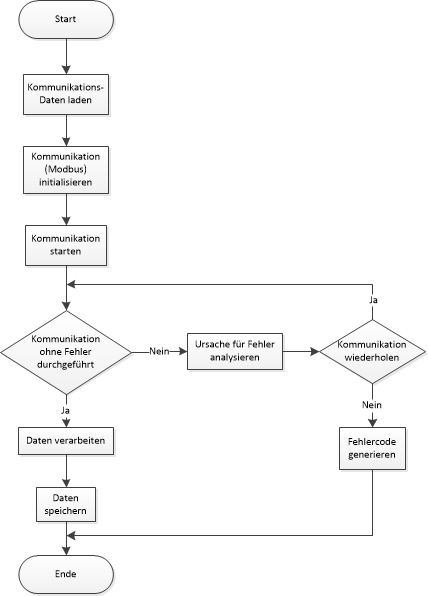
\includegraphics[width=1\textwidth]{./img/Flussdiagramm.png}
\caption{Flussdiagramm des Kommunikationsablaufes}
\label{pic:flussdiagramm_kommunikation}
\end{figure}

\begin{figure}
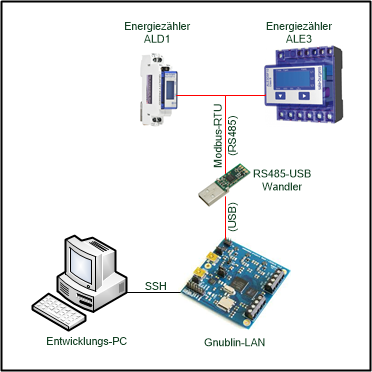
\includegraphics[width=0.9\textwidth]{./img/Labor-Aufbau.png}
\caption{Hardware-Setup der Entwicklungsinfrastruktur}
\label{pic:labor_aufbau}
\end{figure}

\begin{figure}
\centering
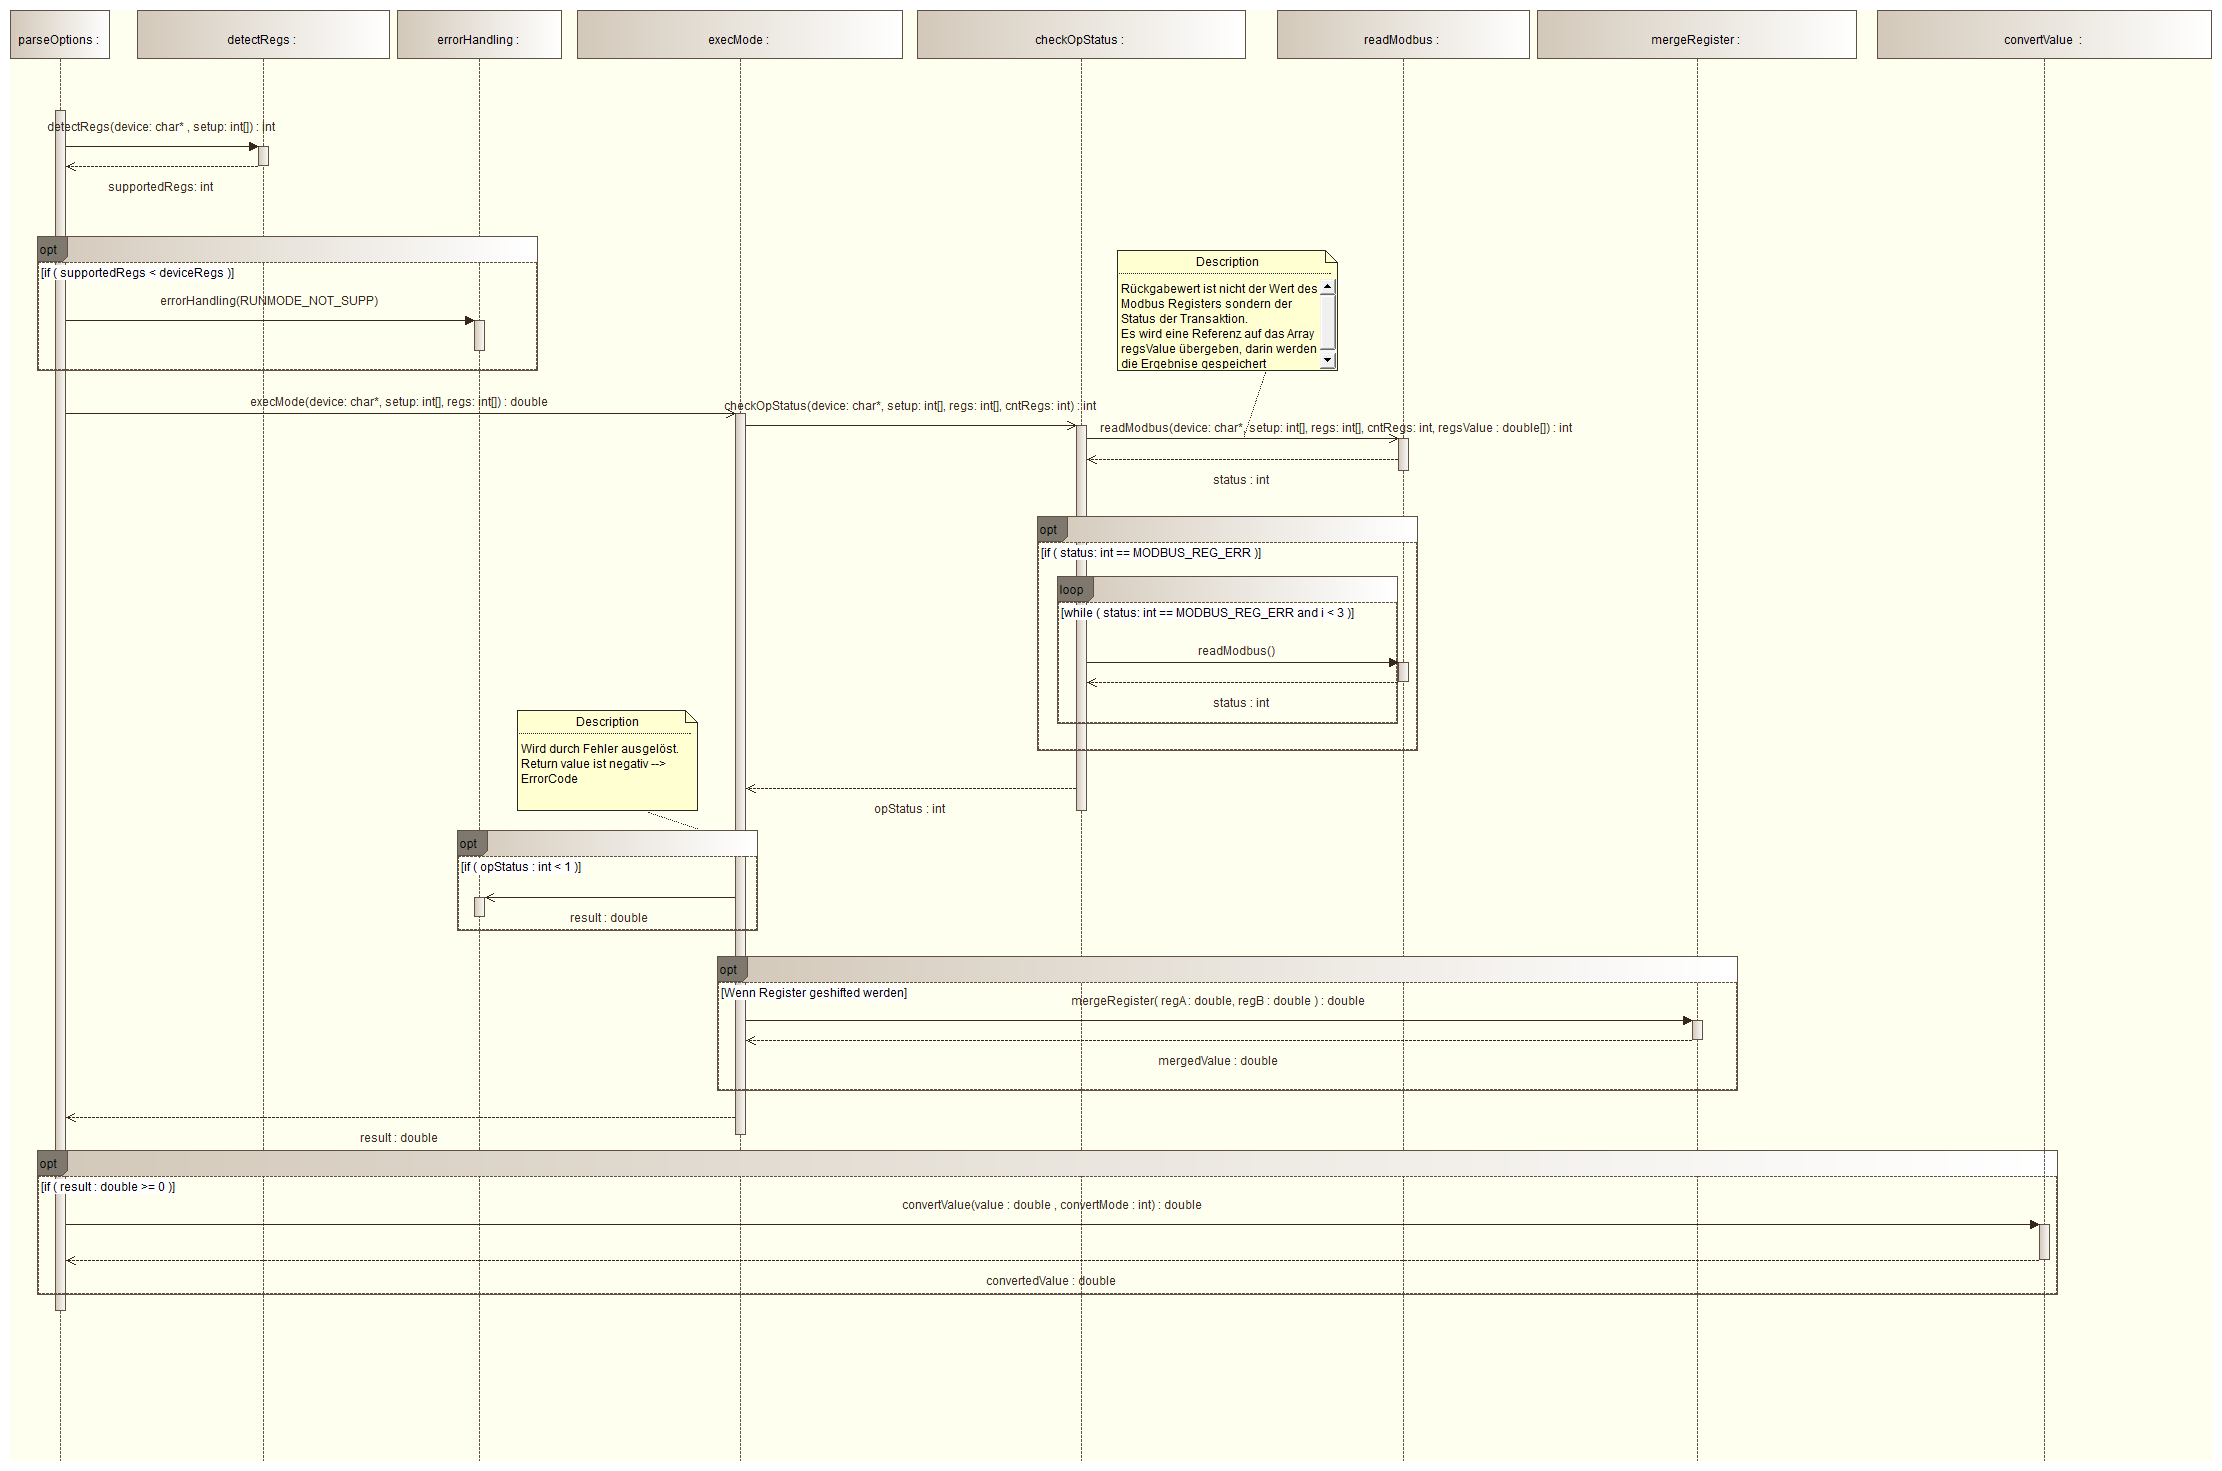
\includegraphics[angle=90,width=1\linewidth]{./img/Sequenzdiagramm_ComModbus}
\caption{Sequenzdiagramm über den Ablauf des Programmes ComModbus}
\label{pic:sequenzdiagramm_comModbus}
\end{figure}

\begin{figure}
\centering
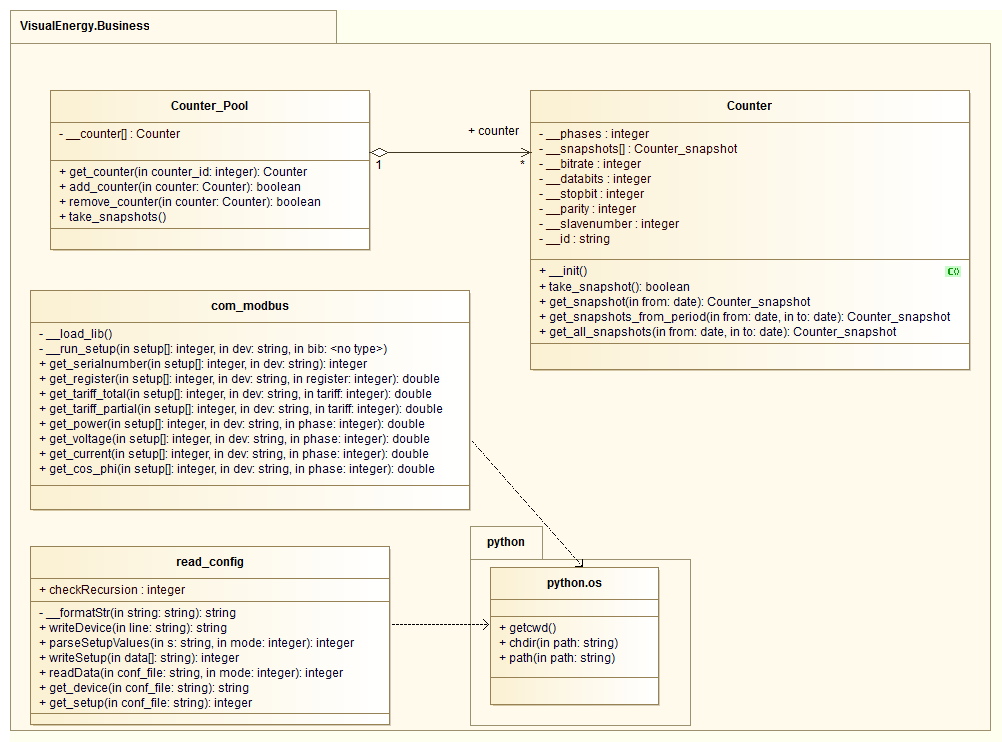
\includegraphics[width=0.9\linewidth]{./img/Klassendiagramm_Business}
\caption{Klassendiagramm der Businessschicht}
\label{pic:klassendiagramm_business}
\end{figure}

\begin{figure}
\centering
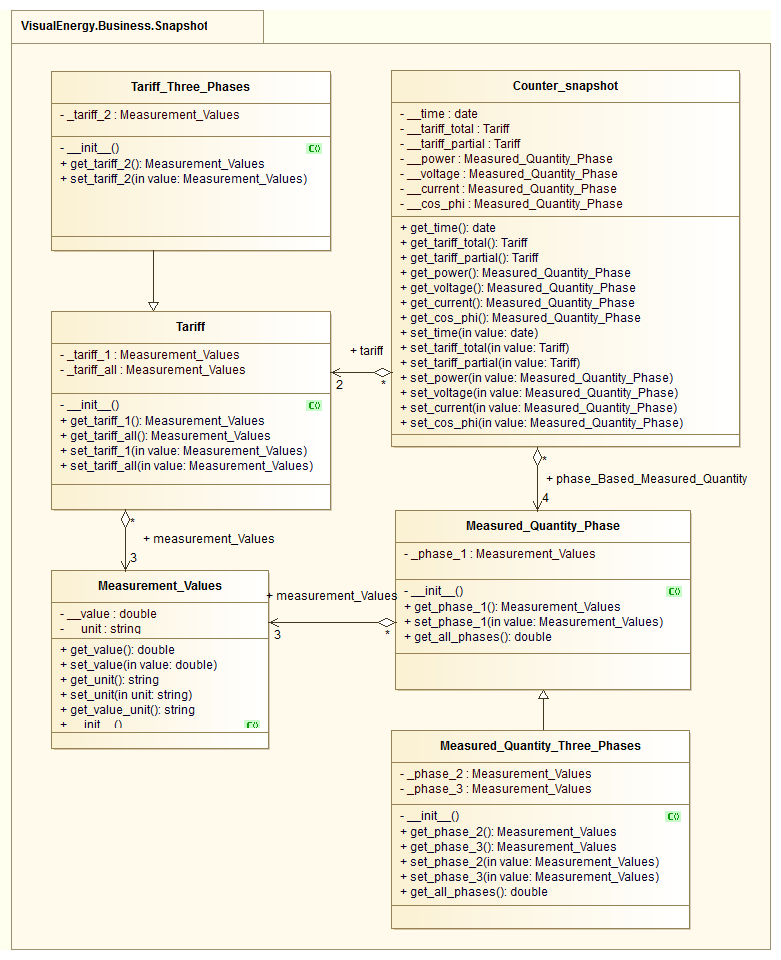
\includegraphics[width=0.9\linewidth]{./img/Klassendiagramm_Snapshot}
\caption{Klassendiagramm des Snapshot-Struktur}
\label{pic:klassendiagramm_snapshot}
\end{figure}

\begin{figure}
\centering
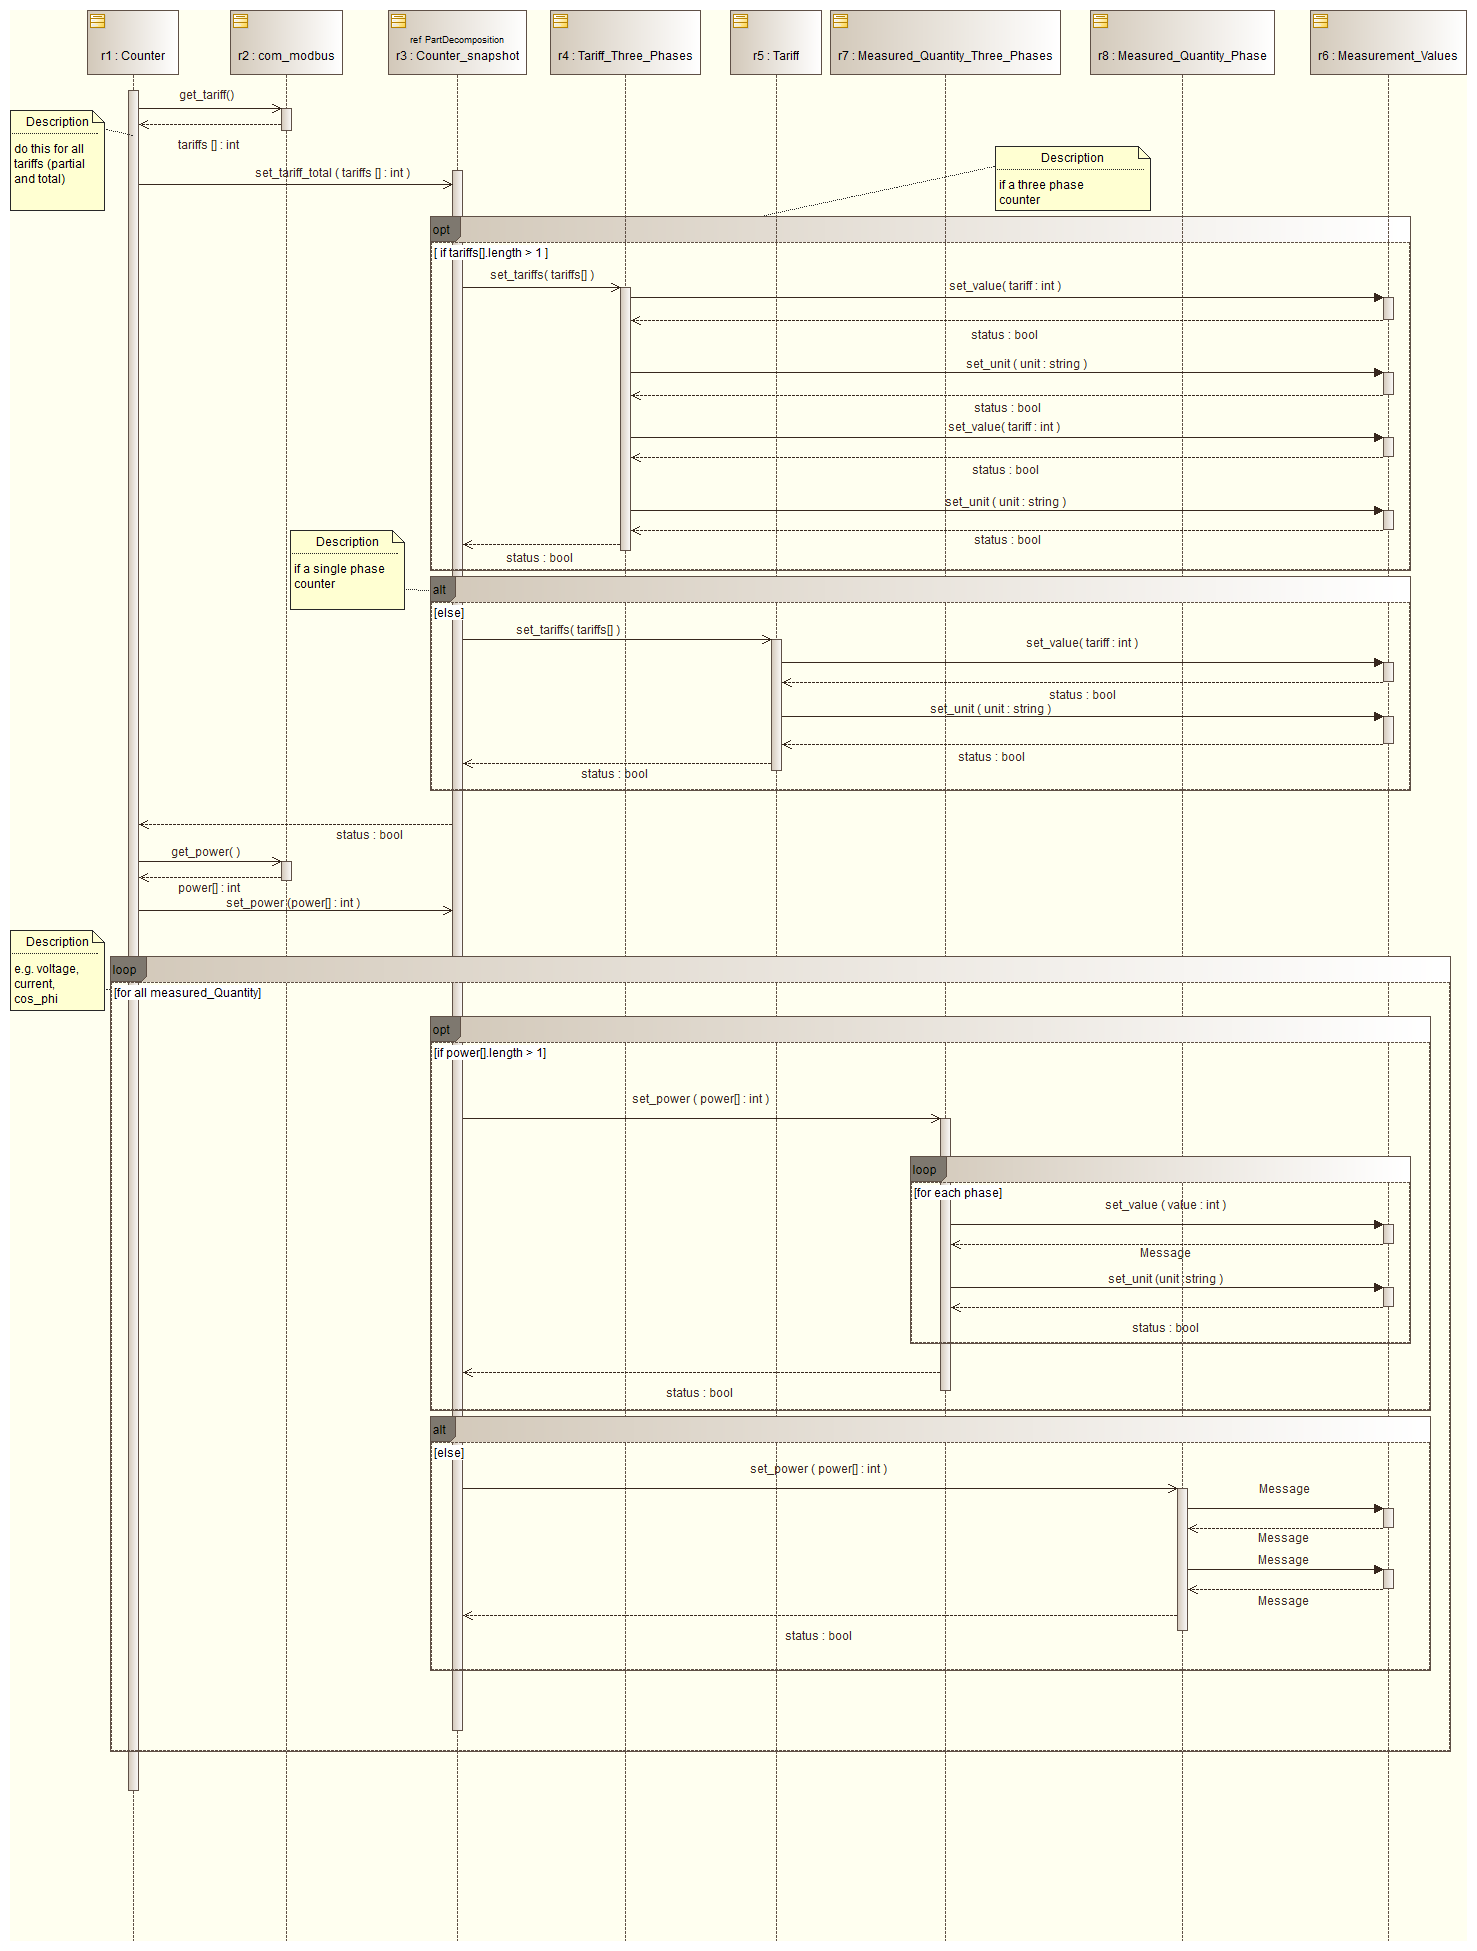
\includegraphics[width=1\linewidth]{./img/Sequenzdiagramm_TakeSnapshot}
\caption{Sequenzdiagramm des Snapshot-Ablaufes}
\label{pic:sequenzdiagramm_takeSnapshot}
\end{figure}


\begin{figure}
\centering
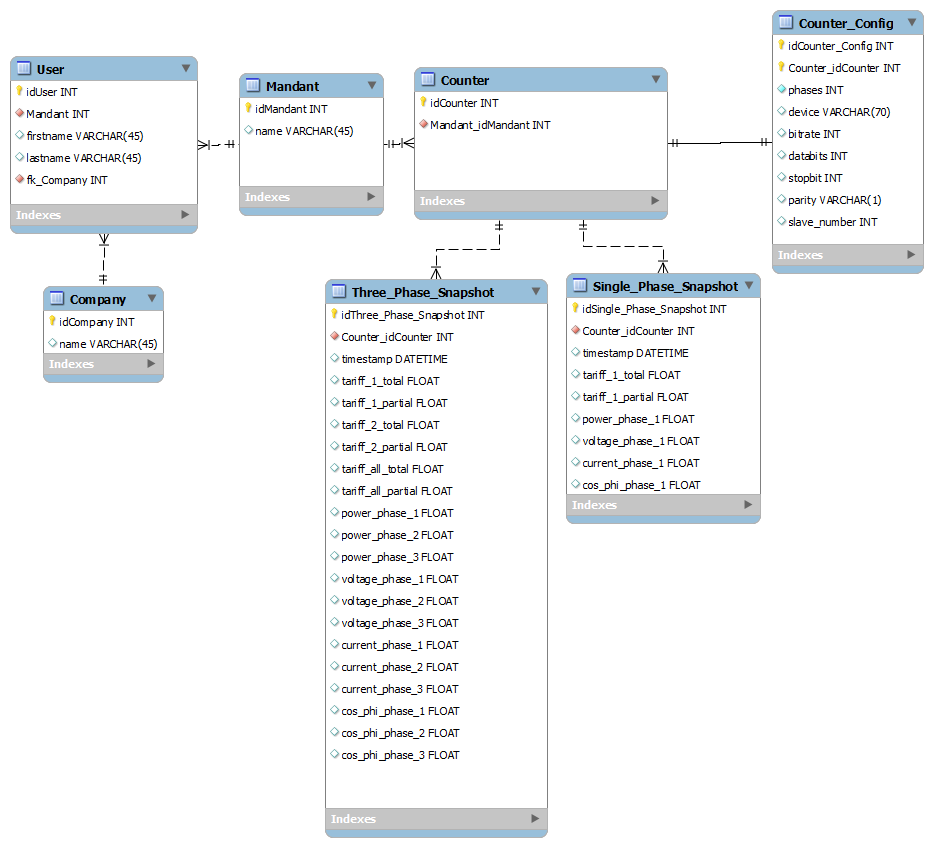
\includegraphics[width=0.9\linewidth]{./img/db_modell}
\caption{Aufbau des Datenbank-Modells}
\label{pic:db_modell}
\end{figure}


\end{document}